\chapter{Mesh generator file specification}
\label{mesh-generators}

\minitoc

The simulator has a flexible structured mesh generator for model
studies, and also a set of import filters for reading in meshes from
geomodelling packages. All the mesh generators read the file
\texttt{mesh}, and write into the directory \texttt{gridding}. The
mesh generator is invoked by typing \texttt{rs mesh}.

The structure of the \texttt{mesh} file is:
\begin{verbatim}
begin MeshGenerator
  % Geometry and topology of the computational mesh
end

begin Sources
  % Placement of sources
end

begin TransmissibilityMethod
  % Coupling coefficients for flow calculations, optional
end
\end{verbatim}
Section~\ref{sec:gg:sources} is about placing fluid sources/sinks in
the mesh, Section~\ref{sec:transmissibility} discusses the
transmissibilities, while the other parts of the chapter concerns the
mesh generation part.

%======================================================================

\csection{Structured mesh generation} 
\label{sec:structured-mesh-generation}

A general structured mesh can be generated with non-uniform element
sizes, topology preserving transformations, alternative numbering
schemes and flexible region and data mappings. The mesh generator
input is a mesh description section with the type
\texttt{StructuredMeshGenerator} specified.

In order to facilitate more flexible input of rock regions and rock
data, boxes can be defined with associated boxed rock region and rock
data subsections:


\begin{verbatim}
begin MeshGenerator
  type StructuredMeshGenerator
  
  dimension 3

  begin Geometry
    ... 
  end

  begin RockRegionMap
    ... 
  end

  begin RockData
    ... 
  end

  % optional
  begin Boxes
    ... 
  end

  % optional
  begin RockRegionBoxed
    ... 
  end

  % optional
  begin RockDataBoxed
    ... 
  end

end
\end{verbatim}
%

%%%%%%%%%%%%%%%%%%%%%%%%%%%%%%%%%%%%%%%%%%%%%%%%%%

\csubsection{Geometry}
\label{sec:geometry-structured}

The \texttt{dimension} keyword specifies the dimension of the mesh. 
This is followed by either \texttt{1}, \texttt{2} or \texttt{3}
representing a 1D, 2D or 3D mesh respectively. If the mesh is 2D, the
domain is part of the $xy$-plane (before any transformations). If it
is 1D, it extends in the $x$-direction. If the dimension is other than
3, the size-keywords described below are affected. 

The \texttt{Geometry} subsection contains specifications for mesh
element numbers and sizes, mesh region mappings, numbering schemes and
transformations. The geometry and mapping specific parameters of the
mesh are given in subsections and keywords (all required) within the
\texttt{Geometry} section:

\begin{verbatim}
begin MeshGenerator

  ... 

  begin Geometry
    ... 
  end

  ... 

end
\end{verbatim}
%

\csubsubsection{Origin}
\label{sec:struct-origin}

The mesh origin is given by the three keywords \texttt{X0},
\texttt{Y0} and \texttt{Z0}. Each keyword is followed by the
coordinate value of the respective direction:
%
\begin{verbatim}
begin MeshGenerator

  ... 

  begin Geometry

    X0  0.0
    Y0  1.0
    Z0  0.0

    ... 

  end

  ... 

end
\end{verbatim}

%

\csubsubsection{Sizes}
\label{sec:struct-sizes}

Mesh element numbers and sizes are defined within one or more uniform
parts in each coordinate direction. This enables non-uniform element
sizes in the complete mesh. Moreover, in the $z$-direction, different
mesh regions can be defined to allow mapping of rock regions. The
number of elements and element sizes of within each part are specified
in the arrays \texttt{Nx}, \texttt{Dx}, \texttt{Ny}, \texttt{Dy},
\texttt{Nz} and \texttt{Dz}. In the example below, there are 2 parts
in the $x$-direction, 1 part in the $y$-direction and 3 parts in the
$z$-direction:

\begin{verbatim}
begin MeshGenerator

  ... 

  begin Geometry

    ... 

    array Nx
      2  3
    end

    array Dx
      2.0  5.0
    end

    array Ny
      5
    end

    array Dy
      1.0
    end

    array Nz
      1  10  1
    end

    array Dz
      -1.0  -20.0  -2.0
    end

    ... 

  end

  ... 

end
\end{verbatim}
%
For the $x$-direction in the example above, the first part contains 2
elements each of length 2.0~$\unit{}{\meter}$, while the second part
contains 3 elements each of length 5.0~$\unit{}{\meter}$.  Observe
that the $z$-direction must be specified with negative values for
\texttt{Dz}.

If the mesh dimension is less than 3, only the element sizes in the
``missing'' dimensions are specified and not the number of elements.
The sizes must be given to ensure consistent volumes and areas. For a
1D mesh, the sizes would be given as follows:
%
\begin{verbatim}
begin MeshGenerator

  ... 

  dimension 1

  begin Geometry

    ... 

    array Nx  
      100  20
    end

    array Dx
      10.0  20.0
  
    array Dy
      2.0
    end
  
    array Dz
      -0.1
    end
  
    ... 

  end

  ... 
  
end
\end{verbatim}


\csubsubsection{Region mapping}
\label{sec:struct-regionmapping}

Rock/fluid properties and rock data can be mapped onto particular
regions of the mesh. These mesh regions are only defined in the
$z$-direction. The region mapping type is given by the keyword
\texttt{RegionMappingType} and is followed by either \texttt{Uniform} or
\texttt{Layer}:
%
\begin{verbatim}
begin MeshGenerator

  ... 

  begin Geometry

    ... 

    RegionMappingType Layer

  end

  ... 

end
\end{verbatim}
%
Using the \texttt{Uniform} value, the complete mesh is defined as a
single mesh region with region index~1. With the \texttt{Layer} value,
regions are defined for each $z$-direction part given in the
\texttt{Geometry} section. This gives region indices $1, 2, \ldots,
\text{numParts}$.

The mesh region indices are used in the \texttt{RockRegionMap} section
to map rock/fluid regions to regions of the mesh and in the
\texttt{RockData} section if the \texttt{Regions} mapping type is
chosen. 

\csubsubsection{Numbering schemes}
\label{sec:numbering-schemes}

The user can specify alternative numbering schemes with the keyword
\texttt{LinearIJKOrdering}. Two numbering schemes are available;
\texttt{NaturalIJKOrdering} and \texttt{D2IJKOrdering}. Example:
%
\begin{verbatim}
begin MeshGenerator

  ... 

  begin Geometry

    ... 

    LinearIJKOrdering D2IJKOrdering

    ... 

  end

end
\end{verbatim}
%
If not specified, the \texttt{LinearIJKOrdering} defaults to
\texttt{NaturalIJKOrdering}. More details on the natural
$ijk$-ordering is given in Section~\ref{sec:natural-orient-numbering}.

\csubsubsection{Transformations}
\label{sec:transformations}

Various transformations can be applied to the mesh. These are all
topology preserving transformations. A transformation is specified
within the \texttt{Transform} section:
%
\begin{verbatim}
begin MeshGenerator

  ... 

  begin Geometry

    ... 

    begin Transform

      type BilinearTransform

      ... 

    end

  end

  ... 

end
\end{verbatim}
%
The keyword \texttt{type} must be followed by the name of the
transform. The name must be correctly capitalised. If the
\texttt{Transform} section is omitted, the default
\texttt{IdentityTransform} is used. 

Valid transformations are
%
\begin{itemize}
\item \texttt{TopDepthTransform}
\item \texttt{TopBottomTransform}
\item \texttt{TranslateDilateTransform}
\item \texttt{PerturbationTransform}
\item \texttt{BilinearTransform}
\item \texttt{AnnulusTransform}
\item \texttt{SkewTransform}
\item \texttt{BipolarTransform}
\end{itemize}


\paragraph{Top depth transformation}

The \texttt{TopDepthTransform} only has an effect for a 3D mesh. For each
$(x,y)$-coordinate of the mesh points, the transformation shifts the
corresponding $z$-coordinate a specified distance $dz$ from the
initial position such that
%
\begin{equation}
  \label{eq:1}
  z(x,y) \leftarrow z(x,y) - dz(x,y).  
\end{equation}
%
Thus, for $dz>0$ the new point location is below the original
location. The $dz(x,y)$ values are specified with an
\texttt{EvenLookupTable2D}:
% 
% Comment on points with (x,y) values extending beyond the domain of
% the lookup-table? 
%
\begin{verbatim}
    begin StructuredTransform
      type TopDepthTransform

      begin TopDepth
        type EvenLookupTable

        Dimension 2

        xMin      0
        xMax     10
        nx        5
	      
        yMin      0
        yMax      1
        ny        3

        array data
          1.0  2.0  3.0  4.0  5.0  % dz(x,y1)
          1.2  2.2  3.2  4.2  5.2  % dz(x,y2)
          1.5  2.5  3.5  4.5  5.5  % dz(x,y3)
        end
        
      end

    end
\end{verbatim}
%


\paragraph{Top/bottom transformation}

The \texttt{TopBottomTransform} only has an effect for a 3D mesh. It
transforms the mesh to conform to given top and bottom surfaces. The
transformation operates on the $z$-coordinates only:
%
\begin{align}
  Z(x,y) & \leftarrow dZ(x,y)/dz \,(z(x,y)-z_t)+Z_t(x,y),
\end{align}
%
where
%
\begin{align}
  dZ(x,y) & = Z_b(x,y) - Z_t(x,y),
\end{align}
%
and $z(x,y)$ is the depth in the non-transformed mesh.

The top surface, $Z_t(x,y)$, and bottom surface, $Z_b(x,y)$, must be
given such that $Z_t(x,y) > Z_b(x,y),\; \forall \;(x,y)$. Moreover,
a reference top depth, $z_t$, and (negative) thickness, $dz$ must be given. Example:
%
\begin{verbatim}
    begin StructuredTransform
      type TopBottomTransform

      dz  -100              % dz must be negative
      ztop 0.0              % reference initial top depth

      begin TopSurface      % Z_t(x,y)
        type EvenLookupTable

        Dimension 2

        ... 

     end

     begin BottomSurface    % Z_b(x,y)
       type EvenLookupTable

       Dimension 2

       ... 

     end
  
  end
\end{verbatim}


\paragraph{Translate-dilate transform}
\label{sec:transl-dilate-transf}

The \texttt{TranslateDilateTransform} is only valid for 3D meshes. It
transforms the mesh to conform to a specified rectangular target
geometry by a simple translation and dilation. For each component,
$x$, of the non-transformed point coordinates the transformation is
%
\begin{align}
  x \leftarrow \frac{\Delta x^t}{\Delta x} (x-x_0)+x_0^t,
\end{align}
%
where $x_0^t$ is the target origin, $\Delta x^t$ is the target length,
and $x_0$ and $\Delta x$ is respectively the origin and the length of
the non-transformed domain. 
%
\begin{verbatim}
    begin StructuredTransform
      type TranslateDilateTransform

      array TargetOrigin
        1.0  10.0  -2.0
      end

      array TargetLengths
        10.0  1.0  -20.0    % negative z-values
      end
  
  end
\end{verbatim}


\paragraph{Perturbation transformation}
\label{sec:pert-transf}

The \texttt{PerturbationTransform} is only valid for 2D and 3D meshes. 
It randomly perturbs the $x$- and $y$-coordinates of internal element
corner points. The transformation is given by
%
\begin{align}
  x_{i,j} & \leftarrow x_{i,j} + \alpha \cdot (\rand - 0.5)\cdot
  \min(x_{i+1,j}-x_{i,j},
  x_{i,j}-x_{i-1,j}), \\
  y_{i,j} & \leftarrow y_{i,j} + \alpha \cdot (\rand - 0.5)\cdot
  \min(y_{i,j+1}-y_{i,j}, y_{i,j}-y_{i,j-1}). 
\end{align}
%
The $z$-coordinate is unchanged. The only user input is the parameter
$\alpha$ specified with the keyword \texttt{Alpha}:
%
\begin{verbatim}
    begin StructuredTransform

      type PerturbationTransform

      Alpha  0.3

    end
\end{verbatim}
%


\paragraph{Bilinear transformation}
\label{sec:bilin-transf}

The \texttt{BilinearTransform} is only has an effect for 2D and 3D
meshes. It transforms the unit square in the $xy$-plane to a general
(flat) quadrilateral specified by its four corner points. If the
initial mesh (logical space) is not the unit square, the corner point
coordinates will not be correct in the resulting mesh. The coordinates
for the target quadrilateral, $\vec{x}_i = (x_i, y_i),\: i=1,\ldots,
4$, must be ordered in correspondence with the unit square corners in
the following way:
%
\begin{align}
  \vec{x}_1 \leftrightarrow (0,0),\\
  \vec{x}_2 \leftrightarrow (1,0),\\
  \vec{x}_3 \leftrightarrow (0,1),\\
  \vec{x}_4 \leftrightarrow (1,1). 
\end{align}
%
For 3D meshes, the $z$-coordinate values are left unchanged. The
format is as follows:
%
\begin{verbatim}
    begin StructuredTransform

      type BilinearTransform

      array x
        0.0  2.0  2.0  4.0  % x1  x2  x3  x4
      end

      array y
        0.0  0.0  3.0  3.0  % y1  y2  y3  y4
      end

    end
\end{verbatim}
%


\paragraph{Annulus transformation}


\paragraph{Skew transformation}


\paragraph{Bipolar transformation}



%%%%%%%%%%%%%%%%%%%%%%%%%%%%%%

\csubsection{Data mapping}
\label{sec:struct-rockregions}


\subsubsection{Rock regions}
\label{sec:rock-regions}

The geometric placement of rock/fluid regions is given within the
\texttt{RockRegionMap} subsection. This contains a set of arrays that
map rock region names to the regions of the mesh. In the example below
the rock region \texttt{SandStone} is mapped to mesh regions
\texttt{1} and \texttt{3} while the \texttt{Shale} is mapped to mesh
region \texttt{2}. 

\begin{verbatim}
begin MeshGenerator

  ... 

  begin RockRegionMap

    array SandStone
      1  3
    end

    array Shale
      2
    end

  end

  ... 

end
\end{verbatim}
%
All numbers in the arrays must be valid mesh region indices. Moreover,
every mesh region must have a rock region mapped to it. 

\subsubsection{Rock data}
\label{sec:struct-rockdata}

In the \texttt{RockData} subsection, porosity, permeability,
conductivity, compressibility and heat capacity can be given. The data
can be specified per element, indicated by type \texttt{Global}, or
per mesh region, indicated by type \texttt{Region}. 

Porosity, \texttt{Poro}, and diagonal permeabilities, \texttt{PermX},
\texttt{PermY}, \texttt{PermZ}, are required. The permeability values
should be given in $[\text{m}^2]$ ($1\: \text{m}^2 = 1.01325\cdot
10^{12}\:\text{Darcy}$). Thermal runs also require the rock heat
capacity, \texttt{C}, and heat conductivity tensor diagonals,
\texttt{CondX}, \texttt{CondY}, \texttt{CondZ}. Optional data are the
off-diagonal permeabilities, \texttt{PermXY}, \texttt{PermXZ},
\texttt{PermYZ}, the off-diagonal rock heat conductivities,
\texttt{CondXY}, \texttt{CondXZ}, \texttt{CondYZ}, and the rock
compressibility, \texttt{Cr}. 

With type \texttt{Global}, the parameters must be given for each
element in the whole domain. The array values follow the element
ordering. The number of values must equal the number of elements,
unless an array contains only one value. Then that value is used for
all elements:
%
\begin{verbatim}
begin MeshGenerator

  ... 

  begin RockData

    type Global

    array Poro
      0.20  0.40  0.13  0.25  0.30
    end

    array PermX   % a single value is duplicated for all elements
      1.0e-8
    end

    include y-and-z-perm.dat

  end

  ... 

end
\end{verbatim}
%
Note also the use of the \texttt{include} keyword above which includes
the data in the file ``y-and-z-perm.dat'':
%
\begin{verbatim}
  array PermY
    100.0  105.0  200.0  250.0  0.1
  end

  array PermZ
    10.0  1.5  25.0  20.0  1.0
  end
\end{verbatim}
%

Choosing the type \texttt{Region}, data must be specified for each
mesh region. In this case the data values are constant for each
element within a mesh region. Example with two mesh regions defined:
%
\begin{verbatim}
begin MeshGenerator

  ... 

  begin RockData

    type Region
  
    begin 1         % data for mesh region 1
      Poro 0.2
      PermX 1.0e-10
      PermY 1.0e-9
      PermZ 5.0e-6
    end
  
    begin 2         % data for mesh region 2
      Poro 0.15
      PermX 1.0e-9
      PermY 2.0e-10
      PermZ 1.0e-11
    end

  end

  ... 

end  
\end{verbatim}



\subsubsection{Mesh boxes}
\label{sec:mesh boxes}

In the \texttt{Boxes} section, input boxes of the mesh can be
specified. Each box is defined with an array of six integers
indicating begin and end element indices for an $(i,j,k)$-numbering of
the mesh. Example of two boxes defined:
%
\begin{verbatim}
begin MeshGenerator

  ... 

  begin Geometry
    ... 
  end

  begin Boxes

    array BoxOfSand  % 4 elements
      2 3  2 2  1 2  % i1 i2  j1 j2  k1 k2
    end

    array ShaleBox   % 6 elements
      1 3  1 1  3 4  % i1 i2  j1 j2  k1 k2
    end

  end

  ... 

end
\end{verbatim}
%


\subsubsection{Boxed rock regions}
\label{sec:boxed-rock-regions}

In the \texttt{RockRegionBoxed} subsection, rock/fluid regions can be
mapped to boxes defined in the \texttt{Boxes} subsection. Example:
%
\begin{verbatim}
begin MeshGenerator

  ... 

  begin RockRegionBoxed
  
    BoxOfSand SandStone
    
    ShaleBox Shale
    
  end

  ... 

end
\end{verbatim}
%
Note that boxed rock regions will overwrite rock regions mapped within
the \texttt{RockRegionMap} subsection. 

\subsubsection{Boxed rock data}
\label{sec:boxed-rock-data}

In the \texttt{RockDataBoxed} section, rock data can be mapped to
boxes defined in the \texttt{Boxes} subsection. The array values
follow the element ordering. The number of values must equal the
number of elements within the box, unless an array contains only one
value. Then that value is used for all elements in the box. Example:
%
\begin{verbatim}
begin MeshGenerator

  ... 

  begin RockDataBoxed

    begin ShaleBox
      array Poro
        0.2                % duplicated for all 6 elements of box
      end

      array PermX
        1.0e-10  1.0e-9  2.0e-11  1.0e-10  1.0e-9  2.0e-11
      end

      array PermY
        2.0e-8             % duplicated for all 6 elements of box
      end

      array PermZ
        include permz.dat  % file permz.dat contains 6 values
      end
    end

    begin BoxOfSand
      array Poro
        0.3  0.15  0.15  0.2
      end

      array PermX
        2.0e-5  1.0e-6  1.0e-5  2.5e-7
      end

      array PermY
        2.0e-5  1.0e-6  1.0e-5  2.5e-7
      end

      array PermZ
        2.0e-5              % duplicated for all 4 elements of box
      end
    end

  end

end
\end{verbatim}

%%%%%%%%%%%%%%%%%%%%%%%%%%%%%%%%%%%%%%%%%%%%%%%%%%%%%%%%%%%%



%%%%%%%%%%%%%%%%%%%%%%%%%%%%%%%%%%%%%%%%%%%%%%%%%%

\csubsection{Natural ordering}
\label{sec:natural-orient-numbering}

The ordering of points, interfaces, elements and connections with the
\texttt{NaturalIJKOrdering} is described here. All input data in the
structured mesh description follow the natural ordering, and indices
always start at 1. This applies when specifying e.g.~source locations.

\subsubsection{Orientations}

The interface numbering is based on orientations. In
Figure~\ref{fig:orient} below, the \texttt{top}, \texttt{bottom},
\texttt{front}, \texttt{back}, \texttt{left} and \texttt{right} mesh
orientation types are defined.
%
\begin{figure}
  \centering
  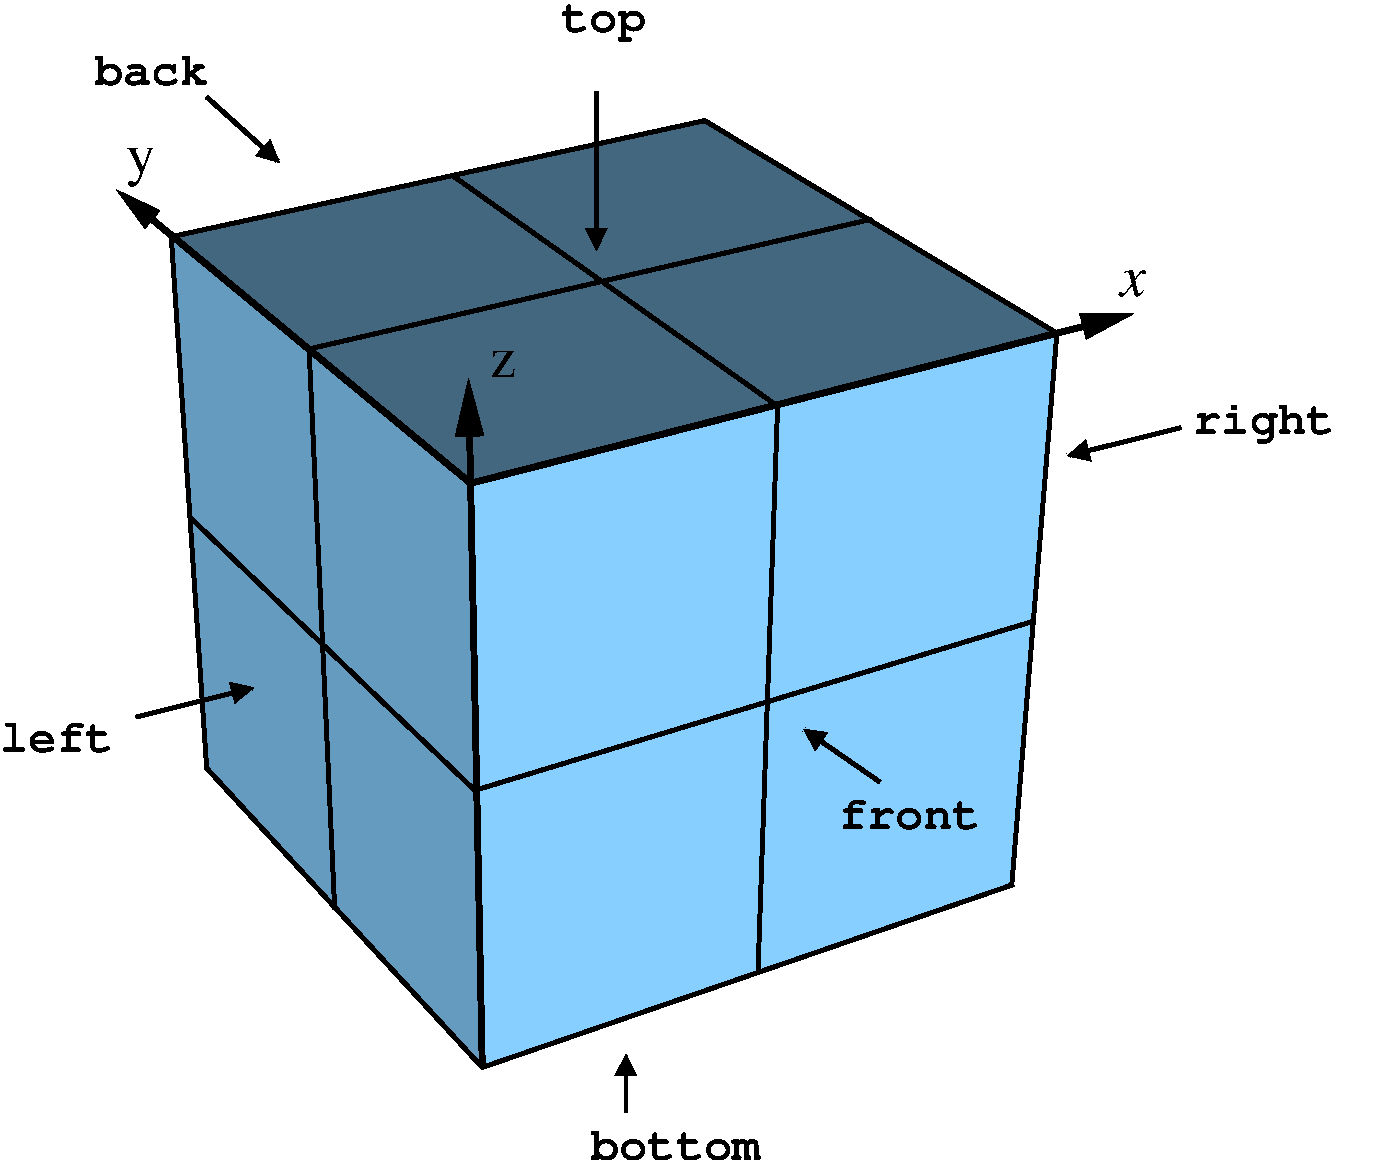
\includegraphics[scale=0.4]{../figures/structorientation}
  \caption{The figure illustrates the six mesh orientation types.}
  \label{fig:orient}
\end{figure}
%

\subsubsection{Points}
%
The naturally ordered points of the structured mesh description are
counted in $xyz$-direction starting at the origin. This is illustrated
in Figure~\ref{fig:cpnumber}. 
%
\begin{figure}
  \centering
  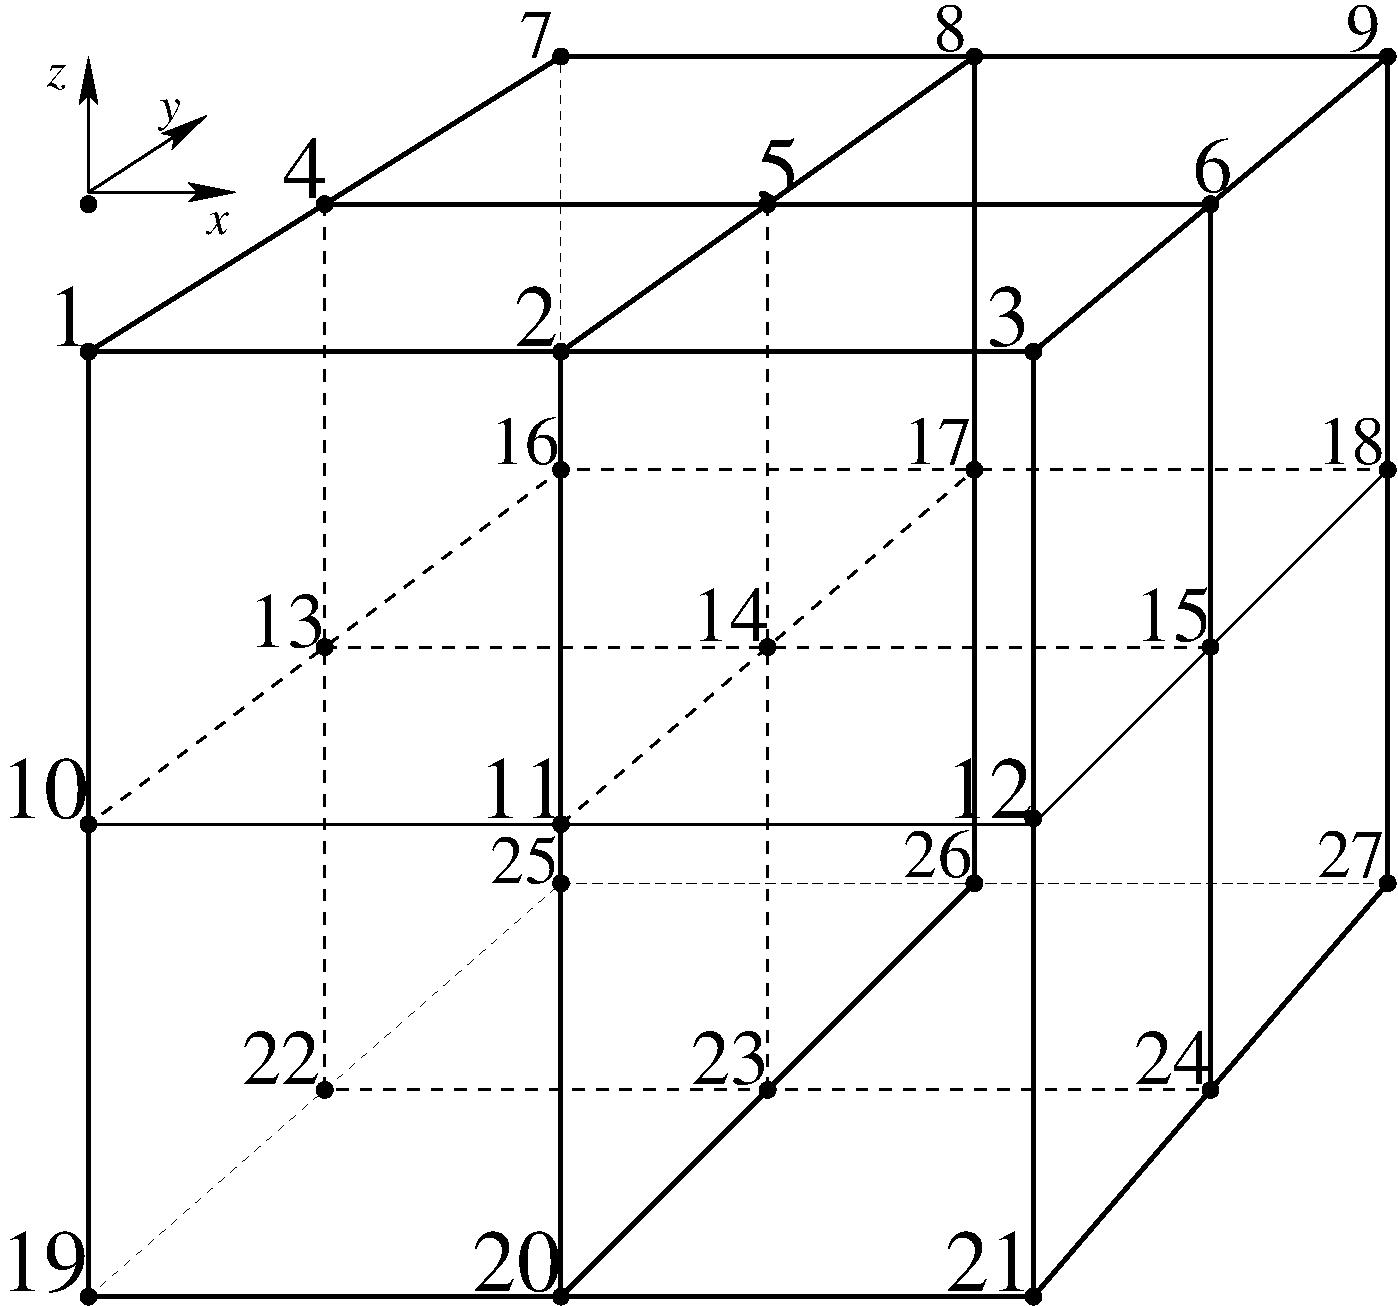
\includegraphics[scale=0.3]{../figures/pointnum}
  \caption{Point numbering for a $2 \times 2 \times 2$-mesh.}
  \label{fig:cpnumber}
\end{figure}
%

\subsubsection{Elements}
\label{sec:elements}

The mesh elements are counted in the $xyz$-direction (negative $z$)
starting with the element at the origin. This is illustrated in
Figure~\ref{fig:cvnumber} for an example $2 \times 2 \times 2$-mesh. 
%
\begin{figure}[htbp]
  \centering
  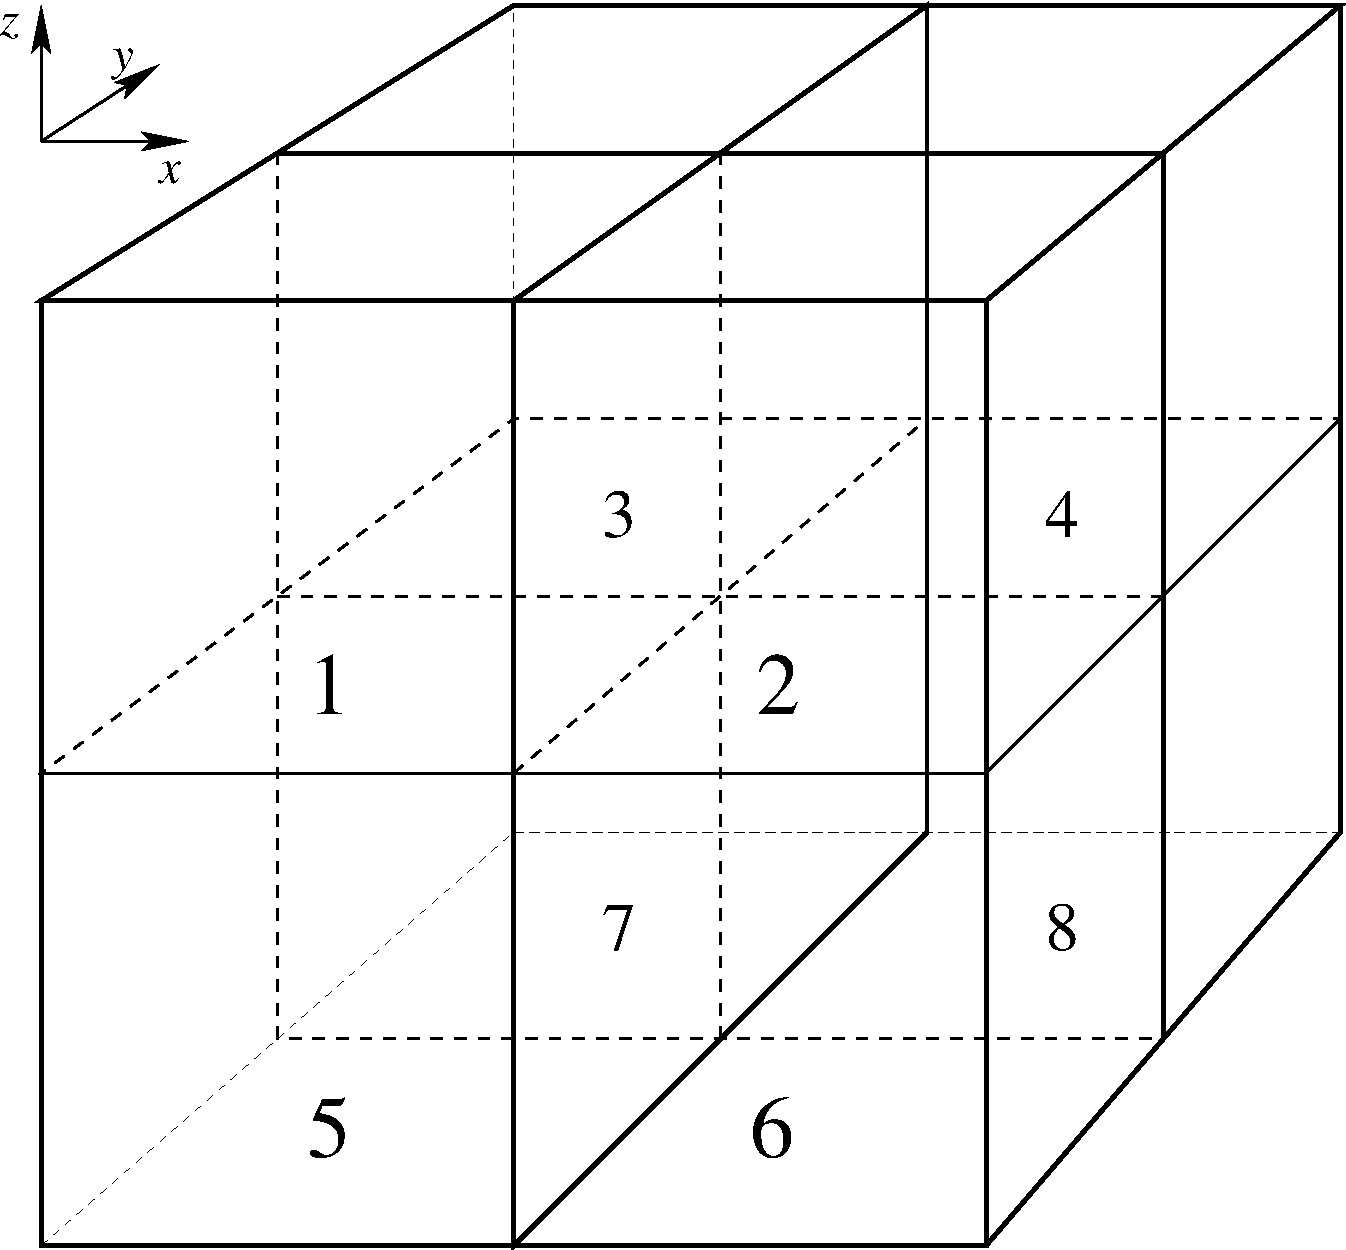
\includegraphics[scale=0.3]{../figures/elementnum}
  \caption{Element numbering for a $2 \times 2 \times 2$-mesh}
  \label{fig:cvnumber}
\end{figure}
%

\subsubsection{Interfaces}
\label{sec:struct-interfaces}

Since each element has a unique set of interfaces, the interfaces are
numbered based on the element numbering. For each element, the
interfaces are numbered consecutively in the order \texttt{Top},
\texttt{Bottom}, \texttt{Front}, \texttt{Back}, \texttt{Left} and
\texttt{Right}. Figure~\ref{fig:intfnumber} below illustrates this in
2D. In this case the interface numbering follows the same order,
except that the top and bottom interfaces do not exist. 
%
\begin{figure}
  \centering
  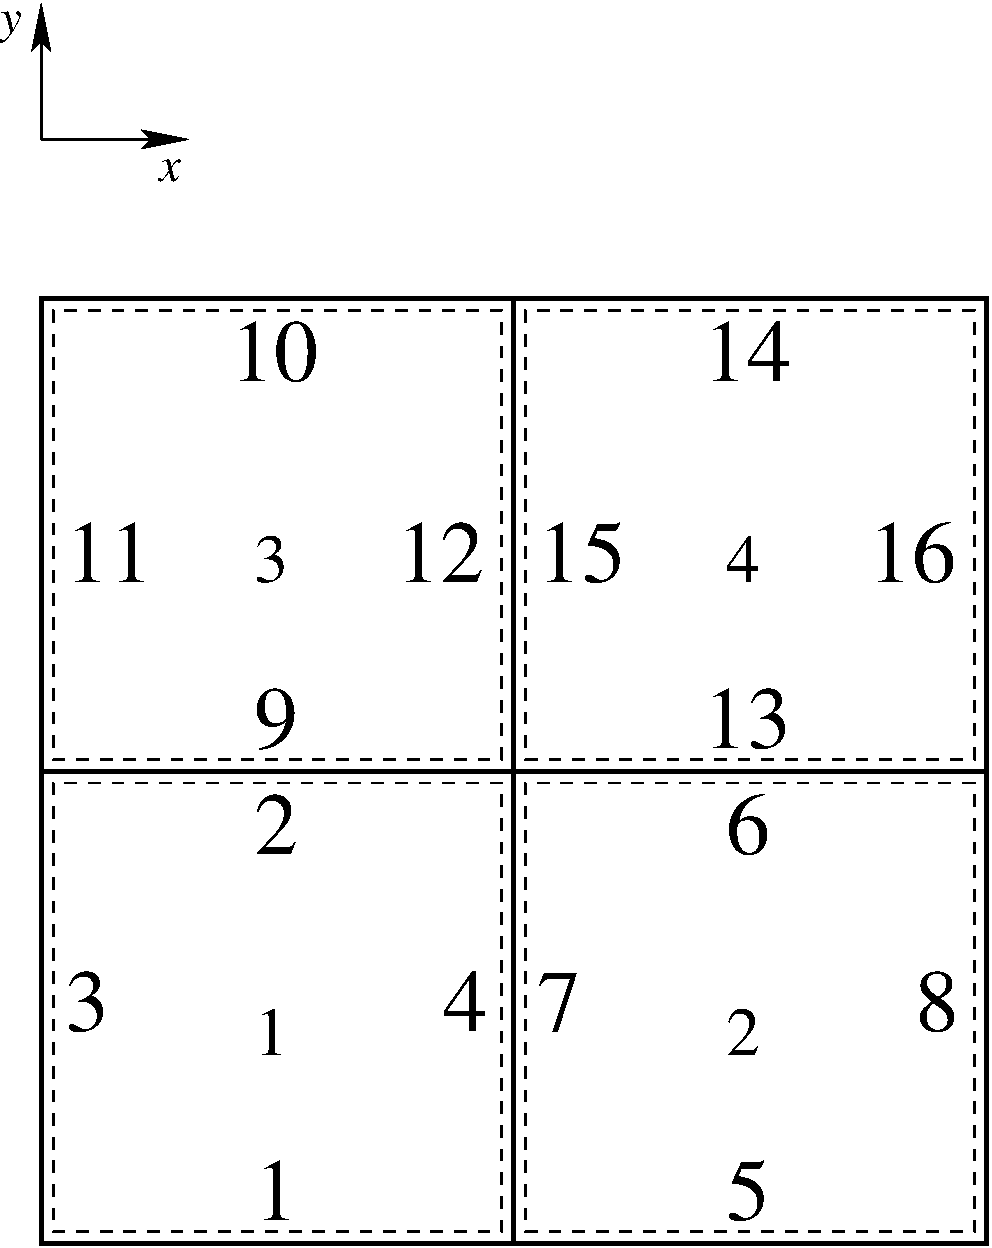
\includegraphics[scale=0.3]{../figures/intfnum2d}
  \caption{Interface numbering for a $2 \times 2$-mesh}
  \label{fig:intfnumber}
\end{figure}
%

\subsubsection{Neighbour connections}

The neighbour connection indexing starts with the top/bottom element
neighbour connections continuing in $xyz$-direction down to the
bottom. This is continued for the front/back neighbour connections,
inwards in $xzy$-direction. The remaining are counted for the
left/right neighbour connections in the $yzx$-direction. This is
illustrated in Figure~\ref{fig:conn-top-bottom},
Figure~\ref{fig:conn-front-back} and Figure~\ref{fig:conn-left-right}
for a $2 \times 2 \times 2$-mesh.
%
\begin{figure}
  \centering
  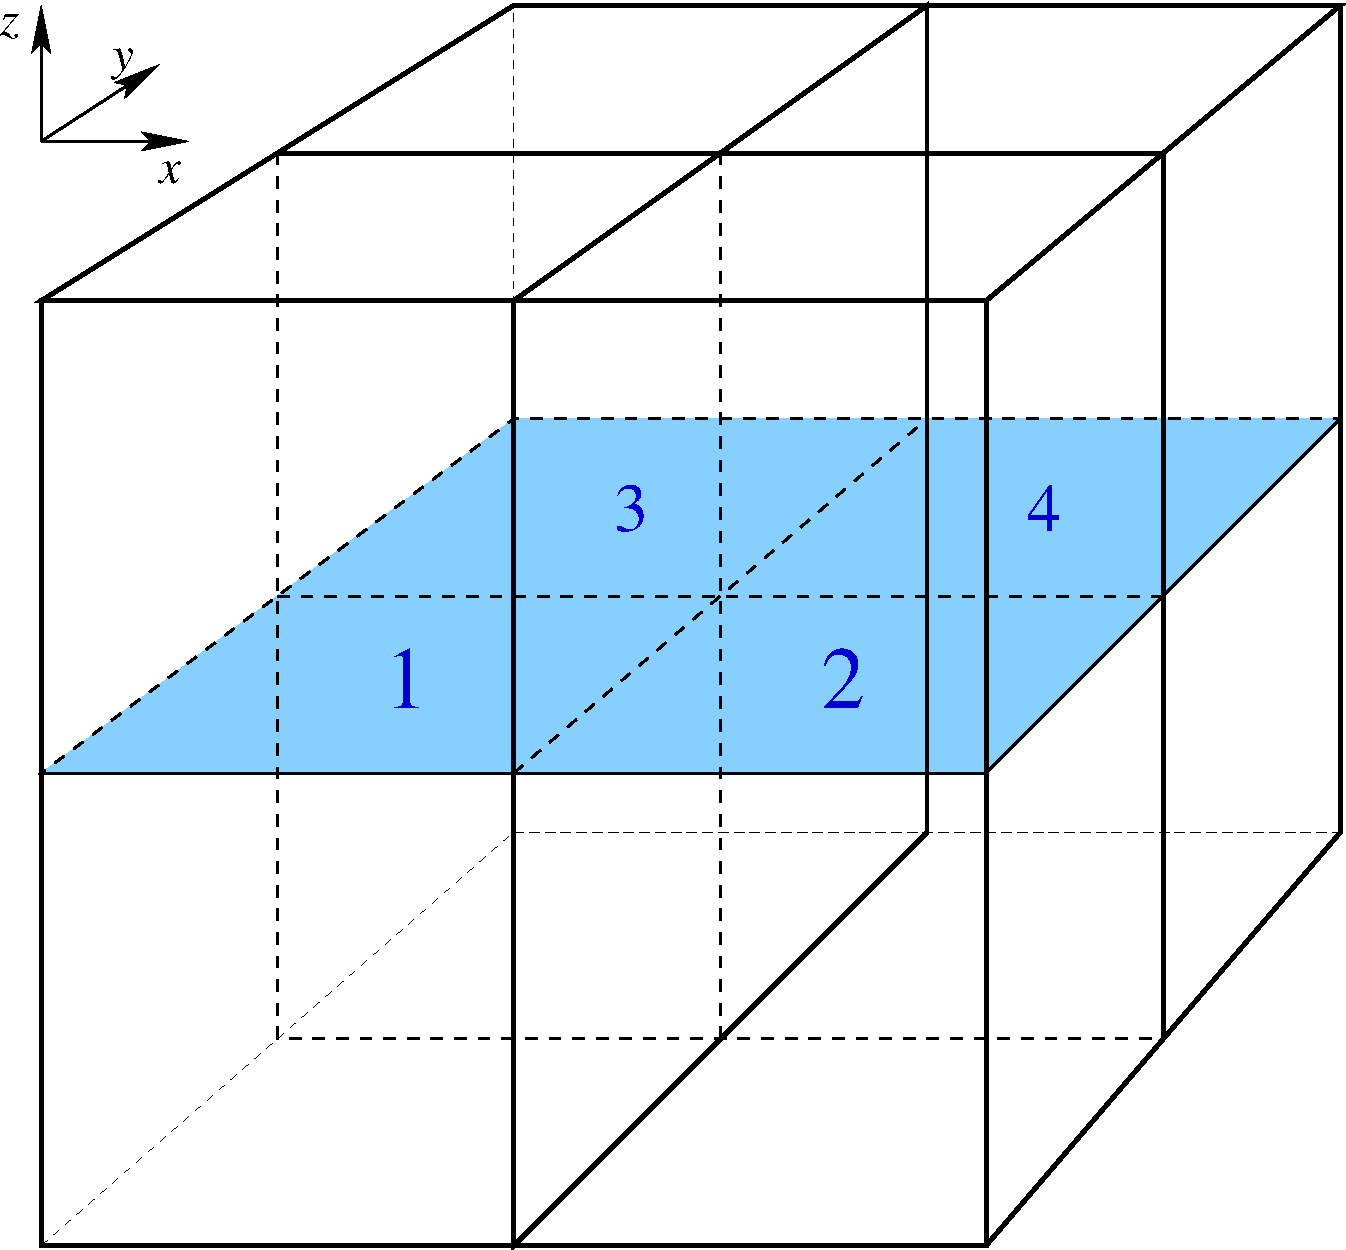
\includegraphics[scale=0.3]{../figures/conn-top-bottom}
  \caption{Neighbour connection numbering for a $2 \times 2 \times
    2$-mesh starting on top.}
  \label{fig:conn-top-bottom}
\end{figure}
%
\begin{figure}
  \centering
  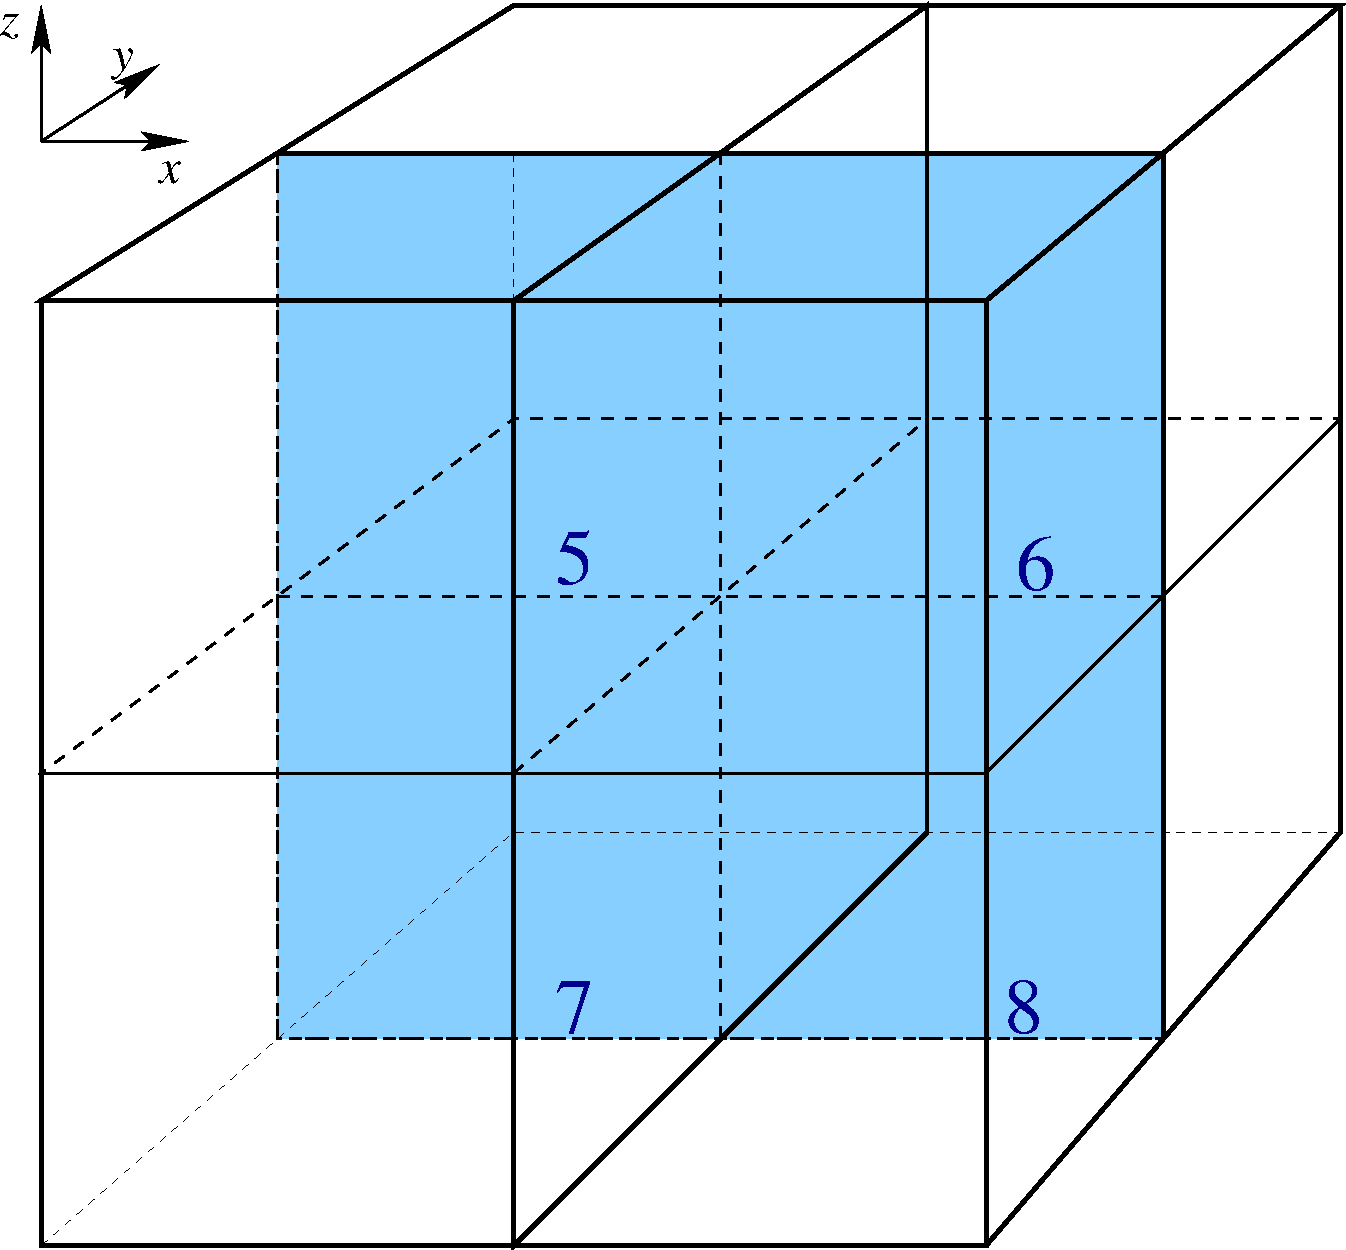
\includegraphics[scale=0.3]{../figures/conn-front-back}
  \caption{Neighbour connection numbering for a $2 \times 2 \times
    2$-mesh continuing from front.}
  \label{fig:conn-front-back}
\end{figure}
%
\begin{figure}
  \centering
  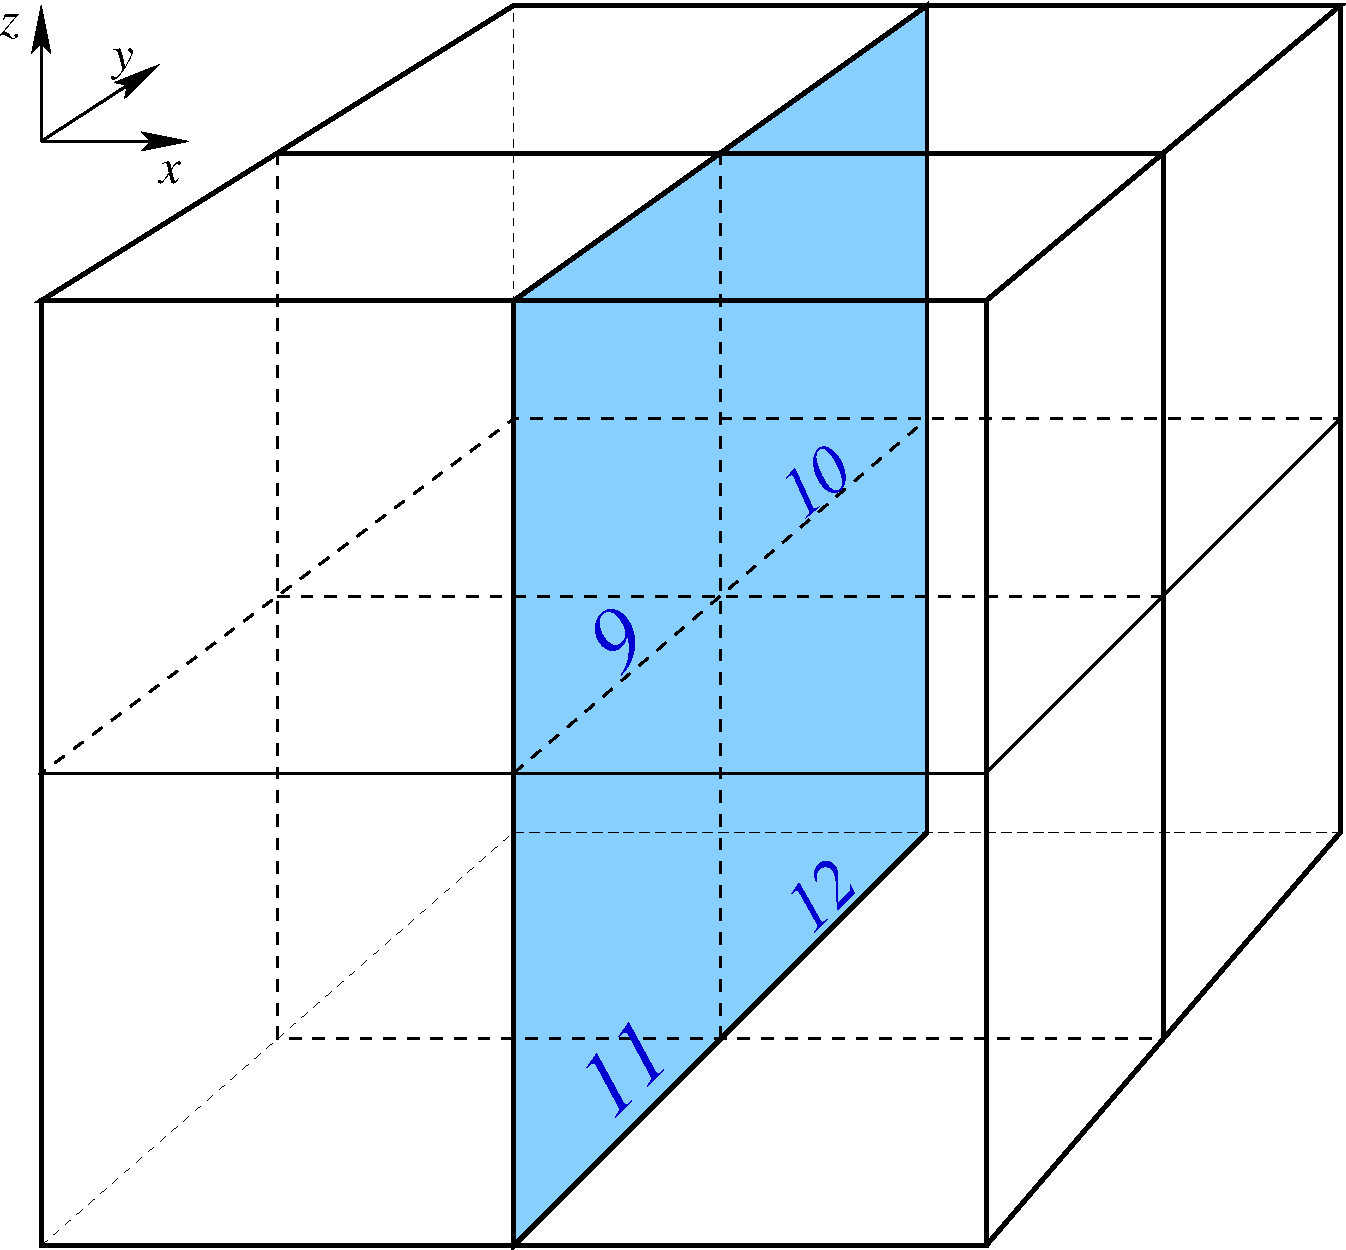
\includegraphics[scale=0.3]{../figures/conn-left-right}
  \caption{Neighbour connection numbering for a $2 \times 2 \times
    2$-mesh finishing from left.}
  \label{fig:conn-left-right}
\end{figure}
%

%%%%%%%%%%%%%%%%%%%%%%%%%%%%%%%%%%%%%%%%%%%%%%%%%%

\csection{Local grid refinement (LGR)}
\label{sec:lgr}

A locally refined mesh will be generated with the keyword
\texttt{LGRMeshGenerator}. In a two-level fashion, a coarse mesh is
first defined. Then, for each desired coarse element, a refinement is
specified. Finally, the meshes in the refined coarse elements are
merged into a composite mesh, discarding non-refined coarse elements:
%
\begin{verbatim}
begin MeshGenerator
  type LGRMeshGenerator

  begin CoarseGeometry
    ...
  end

  begin Refinements

    begin WellRefinement  % refinement with arbitrary but unique name

      array CoarseElementIJK
        1 2 2
      end

      begin FineGeometry
        ...
      end

      begin RockRegionMap
         ...
      end

      begin RockData
        ...
      end

    end

    ...        % more refinements

  end

  begin Transform
    ...     % any transformation valid for the complete LGR mesh
  end

  end

end
\end{verbatim}
%
In contrast to the structured mesh, no alternative numbering scheme
can be given. Also, the coarse mesh does not include data mappings,
and no transformations can be given for the refinements separately.

For each refinement, the mesh geometry is specified within a
rectangular box with starting point at the origin, $(0,0,0)$. This box
is then translated and dilated to fit a target coarse element. There
can only be one refinement per coarse element, and one coarse element
per refinement mesh.

\csubsection{Coarse mesh}
\label{sec:lgr-coarse-mesh}

The \texttt{CoarseGeometry} subsection specifies the coarse mesh
geometry. It follows the same format as for the structured mesh:
%
\begin{verbatim}
begin MeshGenerator
  
  type LGRMeshGenerator

  begin CoarseGeometry

    ... 

  end

  begin Refinements

    ... 

  end

  ... 

end
\end{verbatim}




\csubsection{Refinement mesh}
\label{sec:lgr-fine-mesh}

In the subsection \texttt{Refinements} all refinement meshes are
defined. Each refinement is specified within a separate subsection of
\texttt{Refinements}. The name is arbitrary. In the example below,
three refinements are defined:
%
\begin{verbatim}
begin MeshGenerator
  
  type LGRMeshGenerator

  begin CoarseGeometry

    ... 

  end

  begin Refinements

    begin FaultZone      % refinement 1
                         
      ...                
                         
    end                  
                         
    begin UpperLeft      % refinement 2

      ... 

    end

    begin DamageZone     % refinement 3

      ... 

    end

  end

  ... 

end
\end{verbatim}
%
Note that there must be at least one refinement, and there can not be
more refinements than coarse elements. 

\csubsubsection{Coarse element mapping}
\label{sec:lgr-fine-to-coarse}

The target coarse element is specified within the array
\texttt{CoarseElementIJK} which contains the three integer coarse
element $ijk$-indices. Note that if a specified target coarse element
is already refined, the mesh generation fails. In the
\texttt{FineGeometry} subsection, the numbers of refinement mesh
elements and sizes are specified in addition to the mesh region
mappings. This subsection is similar to the \texttt{Geometry}
subsection for the structured mesh, but contains less data. The
geometry and mapping specific parameters of the mesh are given in
subsections and keywords (all required) within the
\texttt{FineGeometry} section:

\begin{verbatim}
begin MeshGenerator

  ... 

  begin Refinements

    begin DamageZone

      array CoarseElementIJK
        2 1 3
      end

      begin FineGeometry
        ... 
      end

    end

    ... 

  end

  ... 

end
\end{verbatim}
%

\csubsubsection{Sizes}
\label{sec:lgr-sizes}

Mesh element numbers and sizes are defined within one or more uniform
parts in each coordinate direction. This enables non-uniform element
sizes in the complete mesh. Moreover, in the $z$-direction, different
mesh regions can be defined to allow mapping of rock regions. The
number of elements and element sizes of each part are specified in the
arrays \texttt{Nx}, \texttt{Dx}, \texttt{Ny}, \texttt{Dy}, \texttt{Nz}
and \texttt{Dz}. In the example below, there are 2 parts in the
$x$-direction, 1 part in the $y$-direction and 3 parts in the
$z$-direction:

\begin{verbatim}
begin MeshGenerator

  ... 

  begin Refinements

    begin WellZone

      ... 

      begin FineGeometry
    
        array Nx
          2  3
        end
    
        array Dx
          0.05 0.3       % unit cube: 2 * 0.05 + 3 * 0.3 = 1.0
        end              
                         
        array Ny         
          4              
        end              
                         
        array Dy         
          0.25           % unit cube: 4 * 0.25 = 1.0 
        end              
                         
        array Nz         
          1  10          
        end              
                         
        array Dz         
          -0.1  -0.09    % unit cube: 1 * (-0.1) + 10 * (-0.09) = -1.0
        end
    
        ... 
    
      end

    end    % end WellZone refinement

    ...    % more refinements

  end

  ... 
    
end
\end{verbatim}
%
Observe that the $z$-direction must be specified with negative values
for \texttt{Dz}. 

%
\csubsubsection{Refinement region mapping}
\label{sec:lgr-regionmapping}

As for the structured mesh, rock/fluid properties and rock data can be
mapped onto particular regions of each refinement. These refinement
mesh regions are only defined in the $z$-direction. The region mapping
type is given by the keyword \texttt{RegionMappingType} and is followed by
either \texttt{Uniform} or \texttt{Layer}:
%
\begin{verbatim}
begin MeshGenerator

  ... 

  begin Refinements

    begin UpperLeft

      begin FineGeometry
    
        ... 
    
        RegionMappingType Layer
    
      end

    end
    
    ... 

  end

  ... 

end
\end{verbatim}
%
Using the \texttt{Uniform} value, the complete mesh is defined as a
single mesh region with region index~1. With the \texttt{Layer} value,
regions are defined for each $z$-direction mesh part given in the
\texttt{FineGeometry} subsection. 

The mesh region indices are used in the \texttt{RockRegionMap} section
to map rock/fluid regions to regions of the mesh and in the
\texttt{RockData} section if the \texttt{Regions} mapping type is
chosen. 

%%

\csubsection{Data mapping}
\label{sec:lgr-data-mapping}

In the LGR-mesh, data are only given for each refinement. Within each
refinement, the data mapping is performed in exactly the same way as
for the structured mesh. 

\subsubsection{Refinement rock regions}
\label{sec:lgr-rock-regions}

The geometric placement of rock/fluid regions is given within the
\texttt{RockRegionMap} subsection of each refinement. This contains a
set of arrays that map rock region names to the regions of the mesh. 
In the example below the rock region \texttt{SandStone} is mapped to
mesh regions \texttt{1} and \texttt{3} while the \texttt{Shale} is
mapped to mesh region \texttt{2}. 

\begin{verbatim}
begin MeshGenerator

  ... 

  begin Refinements 

    begin FaultZone

      ... 

      begin RockRegionMap
    
        array SandStone
          1  3
        end
    
        array Shale
          2
        end
    
      end
    
      ... 
    
    end 

    ... 

  end

end
\end{verbatim}
%
All numbers in the arrays must be valid refinement mesh region
indices. Moreover, every mesh region must have a rock region mapped to
it. 

\subsubsection{Rock data}
\label{sec:lgr-struct-rockdata}

In the \texttt{RockData} subsection, porosity, permeability,
conductivity, compressibility and heat capacity can be given. The data
can be specified per element, indicated by type \texttt{Global}, or
per mesh region, indicated by type \texttt{Region}. 

Porosity, \texttt{Poro}, and diagonal permeabilities, \texttt{PermX},
\texttt{PermY}, \texttt{PermZ}, are required. The permeability values
should be given in $[\text{m}^2]$ ($1\: \text{m}^2 = 1.01325\cdot
10^{12}\:\text{Darcy}$). Thermal runs also require the rock heat
capacity, \texttt{C}, and heat conductivity tensor diagonals,
\texttt{CondX}, \texttt{CondY}, \texttt{CondZ}. Optional data are the
off-diagonal permeabilities, \texttt{PermXY}, \texttt{PermXZ},
\texttt{PermYZ}, the off-diagonal rock heat conductivities,
\texttt{CondXY}, \texttt{CondXZ}, \texttt{CondYZ}, and the rock
compressibility, \texttt{Cr}. 

With type \texttt{Global}, the parameters must be given for each
element within the whole refinement. The array values follow the
element ordering. The number of values must equal the number of
elements, unless an array contains only one value. Then that value is
used for all elements. Example:
%
\begin{verbatim}
begin MeshGenerator

  ... 

  begin Refinements

    begin DamageZoneHW

      ... 

      begin RockData
    
        type Global
    
        array Poro
          0.20  0.40  0.13  0.25  0.30
        end
    
        array PermX   % a single value is duplicated for all elements
          1.0e-8
        end
    
        include y-and-z-perm.dat
    
      end
    
      ... 

    end    

    ... 

  end

  ... 

end
\end{verbatim}
%
Note also the use of the \texttt{include} keyword above which includes
the data in the file ``y-and-z-perm.dat'':
%
\begin{verbatim}
  array PermY
    100.0  105.0  200.0  250.0  0.1
  end

  array PermZ
    10.0  1.5  25.0  20.0  1.0
  end
\end{verbatim}
%

Choosing the type \texttt{Region}, data must be specified for each
refinement mesh region. In this case the data values are constant for
each element within a refinement mesh region. Example with two mesh
regions defined:
%
\begin{verbatim}
begin MeshGenerator

  ... 

  begin Refinements

    begin FaultZone 

      ... 

      begin RockData
    
        type Region
      
        begin 1         % data for mesh region 1
          Poro 0.2
          PermX 1.0e-10
          PermY 1.0e-9
          PermZ 5.0e-6
        end
      
        begin 2         % data for mesh region 2
          Poro 0.15
          PermX 1.0e-9
          PermY 2.0e-10
          PermZ 1.0e-11
        end
    
      end
    
      ... 

    end

    ... 

  end

  ... 
    
end  
\end{verbatim}


\subsubsection{Refinement mesh boxes}
\label{sec:lgr-mesh boxes}

In the \texttt{Boxes} section, input boxes of each refinement mesh can
be specified. A box is defined with an array of six integers
indicating begin and end element indices for an $(i,j,k)$-numbering of
the mesh. Example of two boxes defined:
%
\begin{verbatim}
begin MeshGenerator

  ... 

  begin Refinements

    begin HighFlowRegion

      ... 

      begin FineGeometry
        ... 
      end

      ... 
    
      begin Boxes
    
        array BoxOfSand  % 4 elements
          2 3  2 2  1 2  % i1 i2  j1 j2  k1 k2
        end
    
        array ShaleBox   % 6 elements
          1 3  1 1  3 4  % i1 i2  j1 j2  k1 k2
        end
    
      end
    
      ... 

    end

    ... 

  end

  ... 
    
end
\end{verbatim}
%


\subsubsection{Boxed rock regions}
\label{sec:lgr-boxed-rock-regions}

In the \texttt{RockRegionBoxed} subsection, rock/fluid regions can be
mapped to boxes defined in the \texttt{Boxes} subsection. Example:
%
\begin{verbatim}
begin MeshGenerator

  ... 

  begin Refinements

    begin ChannelRegion

      ... 

      begin RockRegionBoxed
      
        begin BoxOfSand
          RockRegion SandStone
        end
    
        begin ShaleBox
          RockRegion Shale
        end
    
      end
    
      ... 

    end

    ... 

  end

  ... 
    
end
\end{verbatim}
%
Note that boxed rock regions will overwrite rock regions mapped within
the \texttt{RockRegionMap} subsection. 

\subsubsection{Boxed rock data}
\label{sec:lgr-boxed-rock-data}

In the \texttt{RockDataBoxed} section, rock data can be mapped to
boxes defined in the \texttt{Boxes} subsection. The array values
follow the element ordering. The number of values must equal the
number of elements within the box, unless an array contains only one
value. Then that value is used for all elements in the box.  Example:
%
\begin{verbatim}
begin MeshGenerator

  ... 

  begin Refinements

    begin FaultZone

      ... 

      begin RockDataBoxed
    
        begin ShaleBox
    
          array Poro
            0.2                % duplicated for all 6 elements of box
          end
    
          array PermX
            1.0e-10  1.0e-9  2.0e-11  1.0e-10  1.0e-9  2.0e-11
          end
    
          array PermY
            2.0e-8             % duplicated for all 6 elements of box
          end
    
          array PermZ
            include permz.dat  % file permz.dat contains 6 values
          end
    
        end
    
        begin BoxOfSand
    
          array Poro
            0.3  0.15  0.15  0.2
          end
    
          array PermX
            2.0e-5  1.0e-6  1.0e-5  2.5e-7
          end
    
          array PermY
            2.0e-5  1.0e-6  1.0e-5  2.5e-7
          end
    
          array PermZ
            2.0e-5              % duplicated for all 4 elements of box
          end
    
        end
    
      end

      ... 

    end

    ... 

  end

  ... 
    
end
\end{verbatim}



%%%%%%%%%%%%%%%%%%%%%%%%%%%%%%%%%%%%%%%%%%%%%%%%%%

\csection{Import filters}
\label{sec:import-filters}
The mesh generation tool can also act as an import filter for meshes
from external software. Available formats are
%
\begin{description}
\item[\texttt{DFNMeshImporter}] Converts discrete fracture network
  grid and transmissibility files to native mesh format.
\item[\texttt{SPE10Importer}] Imports SPE 10th comparative study,
  model 2 data, and can extract a subset of it.
\item[\texttt{TriangleMeshImporter}] Reads grid from the Triangle mesh
  generator.
\end{description}
%

\subsubsection{Discrete fracture networks}
\label{sec:discr-fract-netw}

A discrete fracture network grid and transmissibility format from
Stanford University can be converted to the native mesh format by
choosing the type \texttt{DFNMeshImporter} when running the mesh
generator. This is followed by the keywords \texttt{GridFile} and
\texttt{TransFile} which gives the file names for the grid and
transmissibility input files respectively. Example:
%
\begin{verbatim}
begin MeshGenerator
  type DFNMeshImporter

  GridFile  frac2.grid

  TransFile frac2.grid
end
\end{verbatim}
The rock regions are named after the control volume codes. Hence cells
with a code of 1 will belong to \emph{zone1}.

\subsubsection{SPE 10 importer}

This reads the SPE10 Model 2 dataset, and can extract a portion of
it:

\begin{verbatim}
begin MeshGenerator
  type SPE10Importer

  % This file contains the Kx, Ky, and Kz arrays
  PermFile spe10.permeabilities

  % Herein lies a porosity array
  PoroFile spe10.porosities

  array box
    1 60  % I=1..60
    1 220 % J=1..220
    1 85  % K=1..85
  end
end
\end{verbatim}
The arrays within the specified files are flat, that is, no formatting
or anything is necessary. The whole grid has a single rock region,
which is called \emph{rock}.

\subsubsection{Triangle importer}

Reads generated 2D meshes from Triangle:

\begin{verbatim}
begin MeshGenerator
  type TriangleMeshImporter

  % Stemname of the case, defaults to "mesh"
  ProbName mesh

  % Refinement level, defaults to 1
  Refinement 2

  % Fracture transmissibility multiplier, defaults to 1
  FluxMult 0.05

  % Porosity, defaults to 0.25
  Porosity 0.25

  % Permeability, defaults to 1 Darcy
  Permeability 1e-12
end
\end{verbatim}
This reads the files \texttt{mesh.2.poly}, \texttt{mesh.2.ele}, etc.
All cells belong to the same rock region, namely \emph{rock}.

%======================================================================

\csection{Sources}
\label{sec:gg:sources}

To drive the system, fluid sources may be placed around in the mesh.
The placement is done by the mesh generator, while their actions is
defined in the \texttt{run} file.

\begin{verbatim}
begin Sources
  begin WaterInjector
    ...
  end

  begin GasInjector
      ...
  end

  begin Producer
    ...
  end
end
\end{verbatim}

The actual cells to map the sources onto is done by a cell picker.

%----------------------------------------------------------------------

\subsection{Indexed cells}

An indexed cell picker places the source in the given cell indices:

\begin{verbatim}
begin Sources
  begin WaterInjector
    type IndexCellPicker

    array elements
      1 11 21
    end
  end

  ...
end
\end{verbatim}

This places the source \texttt{WaterInjector} in cells 1, 11, and 21.

The line \texttt{type IndexCellPicker} may be omitted, since it
is the default anyway.

%----------------------------------------------------------------------

\subsection{Index ranges}

A range of indices may be compactly expressed as follows:

\begin{verbatim}
begin Sources
  begin GasInjector
    type RangeCellPicker

    start  50
    delta  10
    number  5
  end

  ...
end
\end{verbatim}

This the cells: 50, 60, 70, 80, 90, and 100. If \texttt{delta} is
omitted, it will default to 1.

%----------------------------------------------------------------------

\subsection{Centerpoint}

If you want to specify the source by giving direct coordinates, enter
a statement to use the {\tt CenterPointCellPicker} instead of the
default. Then the $(x,y,z)$ coordinate is given, and the cell closest
to that coordinate is chosen.

\begin{verbatim}
begin Sources
  begin Producer
    type CenterPointCellPicker

    X 100
    Y 50
    Z -10
  end

  ...
end
\end{verbatim}

%======================================================================

\csection{Transmissibility computations}
\label{sec:transmissibility}

The methods of computing transmissibilities for absolute permeability
and heat conductivity can be chosen in the optional
\texttt{TransmissibilityMethod} section.

Available internal methods for computing the absolute permeability
transmissibility are O-method multi-point flux, \texttt{O\_MPFA} and
two-point flux, \texttt{TPFA}. Example:
%
\begin{verbatim}
begin TransmissibilityMethod
  type O_MPFA

  Continuity 1
end
\end{verbatim}
%
The continuity point is set with keyword \texttt{Continuity}. If it
equals 1, the continuity point is at the interface centers, and if it
is equal 0 it is at the element corners. Values in between, such as
0.5, are of course possible. Note that setting the continuity exactly
equal 0 would yield a singular system, hence it cannot be used.

If the \texttt{TransmissibilityMethod} subsection is not given, the
\texttt{O\_MPFA} method is used. The default value for the continuity
point is 1.

And finally, if the mesh is being imported, and it already contains
transmissibilities, new transmissibilities will not be computed.

%%% Local Variables: 
%%% mode: latex
%%% TeX-master: "ug"
%%% End: 
